\documentclass[10pt]{exam}
\usepackage[hon]{template-for-exam}
\usepackage{tikz,multicol,cclicenses,hyperref}
\usetikzlibrary{shadings,shadows,arrows.meta,shapes.geometric}


\title{Rotational Dynamics}
\author{Rohrbach}
\date{\today}

\begin{document}
\maketitle


\section*{Quantities}

\renewcommand{\arraystretch}{2}

\begin{tabular}{p{9em}ccp{6.5em}}
  Concept & Linear/Translational Quantity & Angular/Rotational Quantity & \hfill ``Bridge'' \\ \hline\hline
  cause of acceleration \\[1em] & units: & units:  \\\hline
  inertia \\[1em] & units: & units:  \\\hline
\end{tabular}

\vs

\section*{Moment of Inertia for Extended Objects}

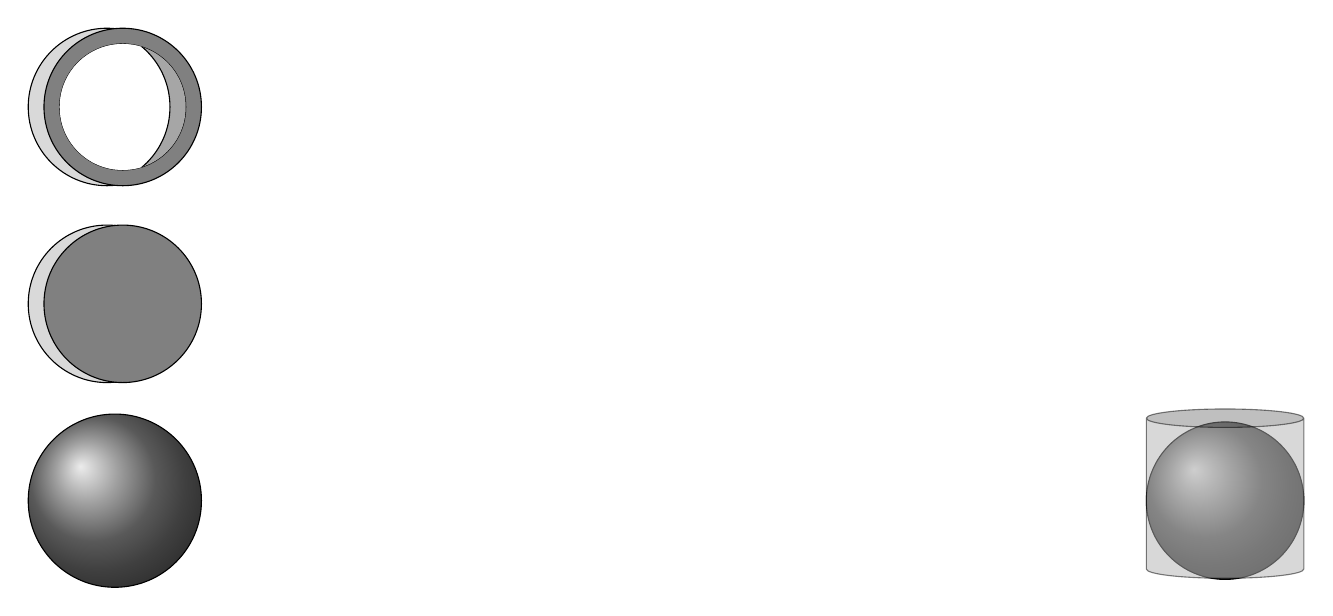
\begin{tikzpicture}
  % \begin{scope}
  %   \draw (0,0) circle (1) (0.1,0.1) circle (1);
  % \end{scope}

  \begin{scope}
    \draw[fill=gray!30] (-0.2,0) circle (1);
    \draw[fill=gray] (0,0) circle (1);
    \draw[fill=white] (0,0) circle (.8);

    \begin{scope}
      \clip (0,0) circle (.8);
      \draw (0,0) circle (.8);
      \fill[gray!70] (-1,-1) rectangle (1,1);
      \draw[fill=white] (-0.4,0) circle (1);
    \end{scope}

  \end{scope}

  % \begin{scope}[shift={(0,-2.5)}]
  %   \node[
  %       cylinder, 
  %       draw=black, 
  %       shape border rotate=90,
  %       minimum width=2cm,
  %       cylinder uses custom fill,
  %       cylinder body fill = gray!60,
  %       cylinder end fill = gray
  %       ] at (0,0) {};
  % \end{scope}

  \begin{scope}[shift={(0,-2.5)}]
    \draw[fill=gray!30] (-0.2,0) circle (1);
    \draw[fill=gray] (0,0) circle (1);
  \end{scope}

  \begin{scope}[shift={(0,-5)}]
    \draw[ball color=gray] (-0.1,0) circle (1.1);
  \end{scope}

  \begin{scope}[shift={(14,-5)}]

    \draw[ball color=gray] (0,0) circle (1);

    \node[
      cylinder, 
      draw=black, 
      semitransparent,
      shape border rotate=90,
      minimum size=2cm,
      minimum height=2.15cm,
      cylinder uses custom fill,
      cylinder body fill = gray!60,
      cylinder end fill = gray
      ] at (-0,0) {};

  \end{scope}
\end{tikzpicture}


\pagebreak

\section*{Practice}

\begin{questions}
  

\question
  Consider the following situation:


  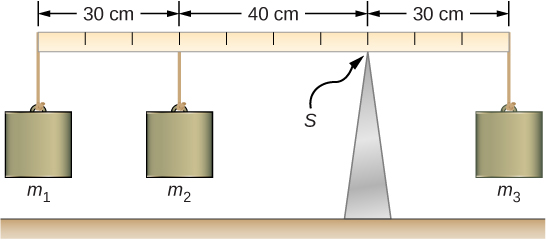
\includegraphics{torque_question.jpg}

  {\footnotesize Image Credit: OpenStax \emph{University Physics}. Authored by: OpenStax CNX. }

  {\footnotesize License:} \cc\hspace{-1em}\ccby  {\footnotesize CC BY: Attribution.}

  {\footnotesize Retrieved 2021-03-02 from \texttt{\href{https://courses.lumenlearning.com/suny-osuniversityphysics/chapter/12-2-examples-of-static-equilibrium/}{https://courses.lumenlearning.com/}} }

  \vspace{1em}

  \begin{parts}
    \part Calculate the net torque about point $S$ if $m_1=10~\text{kg}$, $m_2=20~\text{kg}$, and $m_3=30~\text{kg}$.

    \vs

    \part If you took $m_3$ off, what mass could you replace it with such that the system would balance?

    \vs

  \end{parts}

\question
  A torque of \SI{1.20}{\meter\newton} is applied to a disk of mass 4.80 kg and radius 30 cm until it reaches a rotational speed of 10,300 rpm. Through how many revolutions does the disk rotate during this process?
  \vs

\end{questions}








\end{document}